% REV00 Tue 20 Jul 2021 08:12:01 WIB
% START Tue 20 Jul 2021 08:12:01 WIB

\chapter{Ketiga}

% 11
\begin{figure}[htbp]
% h: here, where the figure appears in the text (use can always just use [h] )
% t: top,  top of the current page.
% b: bottom of the current page.
% p: page, top of the next available float space (sometimes end up being the end of the document).
\centerline{
\includegraphics[scale=0.9]{01-03-01}}
\caption{Ustadz Satiri. Sumber: FB Satiri M Zen.}
\label{01-03-01}
\end{figure}
%

Kata orang bijak, the time you enjoy to waste is not wasting time… Itu artinya kita memang butuh bersenang senang untuk menambah kekuatan…

Di bulan ketujuhnya yang merdeka, Tuhan menurunkan gurunya yang kedua: Mas Paijo. (Tentu saja saya juga tidak tahu nama sebenarnya). Bujang dari Jawa ini kebetulan mengontrak rumah tidak jauh dari rumah Satiri. Pagi ia bertugas sebagai guru muda di SMP Negeri 66 Kebayoran Lama. Sore anak-anak juga suka main di rumahnya. Satiri remaja tentu tidak mau ketinggalan untuk berkenalan dengan orang baru ini. Langsung ia membombardir dengan belasan pertanyaan:

"Mas Paijo kampungnya di Jawa yah?"

"Mas Paijo kerja di mana?"

"Mas Paijo tahu Australia sama Rusia?"

Hanya dalam sekali pertemuan itu sajalah Paijo segera tahu bahwa Satiri ini berbeda. Mengajar Satiri yang banyak bertanya menjadi hiburan tersendiri baginya. Entah bagaimana, berhitung (matematika), bahasa Inggris dan pengetahuan umum menjadi subyek utama obrolan mereka setiap sore untuk berminggu-minggu kemudian.

Datanglah masa untuk penerimaan murid SMP awal tahun pelajaran 1973. Saat itu awal triwulan dimulai bukan Januari. Kita belum mengenal sistem semester. Menghadaplah Paijo, guru muda yang berbangga kepada babanya Satiri. Paijo tentu tahu keadaan keluarga Satiri, sehingga dia memilih (atau tepatnya Tuhan memilihnya) untuk mengambil inisiatif.

% 11
\begin{figure}[htbp]
% h: here, where the figure appears in the text (use can always just use [h] )
% t: top,  top of the current page.
% b: bottom of the current page.
% p: page, top of the next available float space (sometimes end up being the end of the document).
\centerline{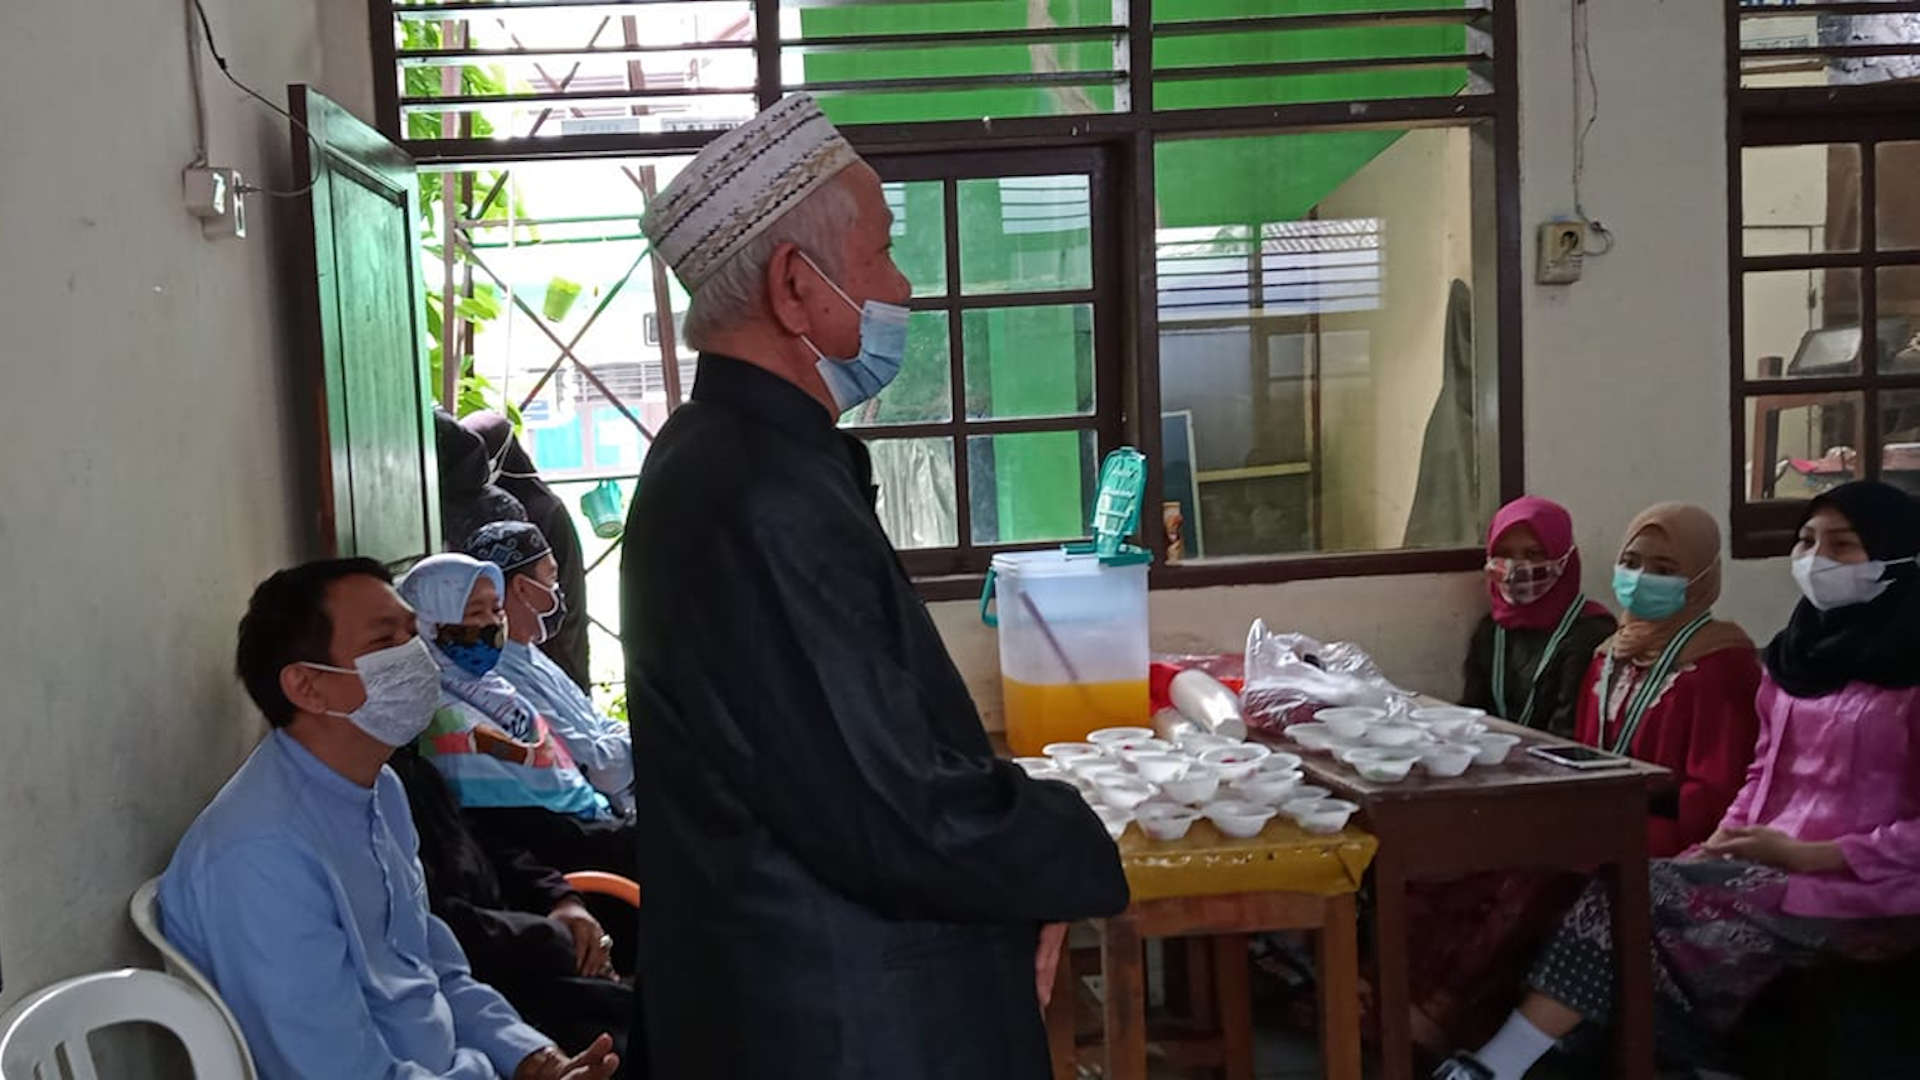
\includegraphics[scale=1.0]{01-03-02}}
\caption{Kepala sekolah almarhum Satiri saat sekolah dasar waktu itu bernama sekolah penampungan. Di daerah rawa belong (Ahmad Muttaqin)}
\label{01-03-02}
\end{figure}
%
“Pak, ini anaknya pintar. Boleh ya saya masukkan ke sekolah saya?”

“Iya terserah elu aja. Kita mah kagak gableg duitnya” (It’s all up to you. We don’t have the money for it…)

Dibawalah Satiri ke SMPN 66, didaftarkan dengan uang pribadinya. Ini hebat betul. Mengapa? Karena untuk berpuluh tahun juara-juara di sekolah itu didominasi anak-anak kaya, cerdas luar biasa, keturunan Tionghoa. Tidak salah kalau Paijo berbangga. Mengapa? Karena murid kecilnya itu kemudain terbukti selalu menjadi juara umum hingga lulus SMP.

Bagaimana Satiri membiayai sekolahnya? Ikut keliling berdagang kembang di sore hari, meniti jejak babanya. Hanya itu yang ia tahu cara mencari nafkah. Lainnya, ia selalu mendapat jajan dari teman-teman yang sering dibantunya belajar.

Dia tidak pernah pelit dengan ilmunya.

Mendekati akhir SMP, Satiri hanya bisa menerawang. Hatinya tidak pasti apa yang kemudian akan datang kepadanya.

Karena Satiri mendobrak tradisi juara, para guru dengan spontan mengumpulkan uang dan buku tulis buat Satiri. Yang tak kalah gembira adalah bapak Kepala Sekolah, yang dengan uang para guru itu membawa Satiri untuk mendaftar di SMA Negeri XI (Sekarang SMAN 70), Bulungan, Jakarta Selatan. SMA terbaik nasional pada masanya. (Kebetulan juga abangku yang tertua lulusan SMA itu, dan setelah ia lulus ia diterima sekaligus di tiga universitas besar nasional, yang kemudian dia memilih masuk Elektro ITB).

Satiri sebetulnya amat sangat ragu masuk ke sekolah elit itu. Dia tidak mampu membayangkan entah uang sekolahnya dari mana. Dan di sana semua anak orang kaya. Pandangannya kosong. Tapi Tuhan mencatat kata “Australia sama Rusia” itu...
\\[10pt]

Sumber tulisan asli \url{https://www.facebook.com/reno.alamsyah.94/posts/10226517785116973}

